\documentclass{article}
\usepackage{geometry}
\usepackage{paralist}
\usepackage[T1]{fontenc}
\usepackage{reledmac}
\usepackage{changepage}

\usepackage{pgfplots}
\usepackage{tikz}
\usetikzlibrary{positioning}
\usetikzlibrary{shapes.geometric, arrows}
\tikzstyle{arrow} = [thick,->,>=stealth]

\usepackage{fancyhdr}
\fancyhead[L]{
	\begin{tabular}{l}
		\LARGE \textbf{\textsc{Distributed Algorithms}} \\
		\Large Exercise 01
	\end{tabular}
}
\fancyhead[R]{
	\begin{tabular}{r}
		16-124-836 \\
		Marcel \textsc{Zauder}
	\end{tabular}
}
\renewcommand{\headrulewidth}{0.4pt}
\fancyfoot[C]{\thepage}
\renewcommand{\footrulewidth}{0.4pt}

\usepackage{hyperref}

\begin{document}
	\pagestyle{fancy}
	
	\section*{1.2 Describing Dependable Systems}
	\begin{adjustwidth}{2em}{2em}
		We will consider the distributed system embedded in an autopilot of an aircraft: \\
		\begin{center}
			\begin{tabular}{|ccccc|}
				\hline 
				& & & & \\
				\multicolumn{5}{|c|}{\Large \textbf{Autopilot of an Aircraft (C)}} \\
				& & & & \\
				&
				\begin{tabular}{|c|}
					\hline
					\\
					\textit{Flight Instructions} \\
					\\
					\hline
				\end{tabular}
				&
				&
				\begin{tabular}{|clc|}
					\hline
					& & \\
					\multicolumn{3}{|c|}{\textit{Flight Information (B)}} \\
					& & \\
					&
					\begin{tabular}{|l|}
						\hline
						Speed \\
						\hline
					\end{tabular}
					& \\
					&
					\begin{tabular}{|l|}
						\hline
						Orientation/Position \\
						\hline
					\end{tabular}
					& \\
					&
					\begin{tabular}{|l|}
						\hline
						Altitude (A) \\
						\hline
					\end{tabular}
					& \\
					& & \\
					\hline
				\end{tabular}
				& \\
				& & & & \\
				\hline
			\end{tabular}
		\end{center}
		
%Für Bäsi
\begin{center}
	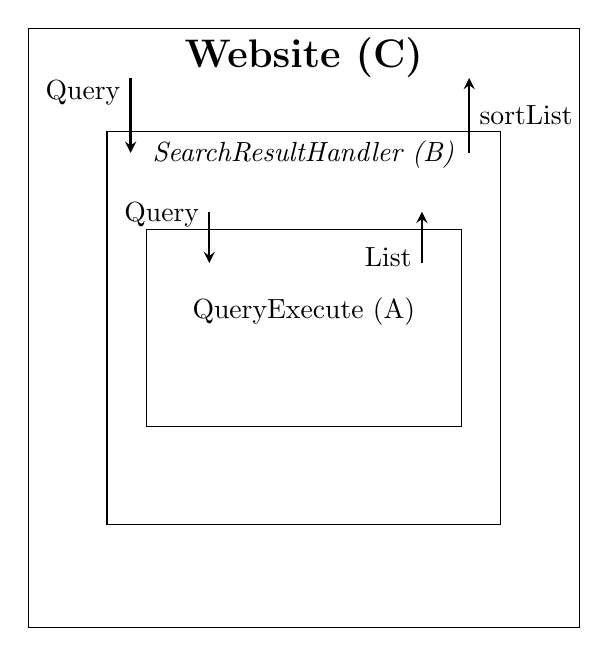
\begin{tikzpicture}
		%Rectangles
		\node(rect) [draw, thin, text depth = 7cm, minimum height = 7cm, minimum width = 7cm] (main){\Large \textbf{Website (C)}};
		\node[draw, thin, text depth = 4.5cm, minimum height = 4cm, minimum width = 5cm] at (main.center) (sub){\textit{SearchResultHandler (B)}};
		\node[draw, thin, text depth = 0.5cm, minimum height = 2.5cm, minimum width = 4cm] at (sub.center){QueryExecute (A)};
		
		%Nodepoints
		\node [] (queryOut) at ([yshift=3.3cm, xshift=-2.2cm]main.center) {};
		\node [] (queryIn) at ([yshift=2.1cm, xshift=-2.2cm]main.center) {};
		\node [] (sortedListIn) at ([yshift=3.3cm, xshift=2.1cm]main.center) {};
		\node [] (sortedListOut) at ([yshift=2.1cm, xshift=2.1cm]main.center) {};
		
		\node [] (queryOut2) at ([yshift=1.6cm, xshift=-1.2cm]main.center) {};
		\node [] (queryIn2) at ([yshift=0.7cm, xshift=-1.2cm]main.center) {};
		\node [] (listIn) at ([yshift=1.6cm, xshift=1.5cm]main.center) {};
		\node [] (listOut) at ([yshift=0.7cm, xshift=1.5cm]main.center) {};
		
		%Lines
		\draw[arrow] (queryOut) -- node[ anchor= south east ]{Query} (queryIn);
		\draw[arrow] (queryOut2) -- node[ anchor=south east ]{Query} (queryIn2);
		\draw[arrow] (sortedListOut) -- node[ anchor=west ]{sortList} (sortedListIn);
		\draw[arrow] (listOut) -- node[ anchor=north east ]{List} (listIn);
		
	\end{tikzpicture}		
\end{center}				
		
	\end{adjustwidth}
	
\end{document}